\section{Results}
\subsection{Parameters}

\begin{figure}
\centering

\includegraphics[width = 7.5cm]{results/smileface.jpg}
\vspace{0.5mm}
\caption{ Denoising results using different values of $\sigma_r$ with other parameters fixed.}
\label{Fig:sigma}
\end{figure}


%\begin{figure*}
%\centering
%
%\subfigure
%{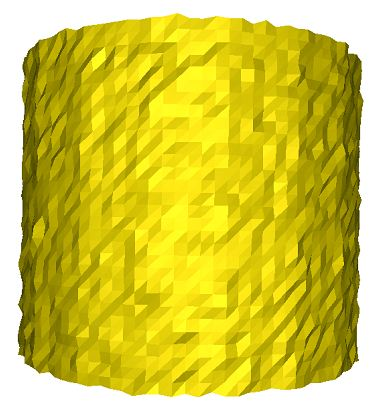
\includegraphics[width = 1.8cm]{results/Prism0.1/snapshot00.jpg}}
%\subfigure
%{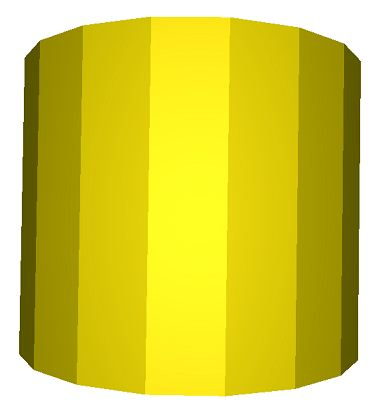
\includegraphics[width = 1.8cm]{results/Prism0.1/snapshot01.jpg}}
%\subfigure
%{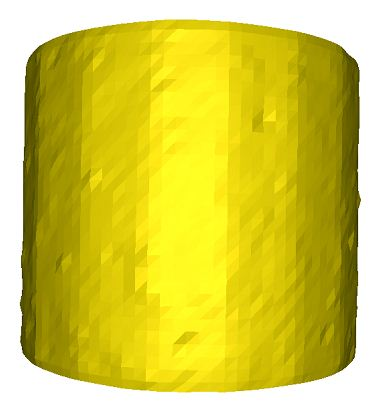
\includegraphics[width = 1.8cm]{results/Prism0.1/snapshot02.jpg}}
%\subfigure
%{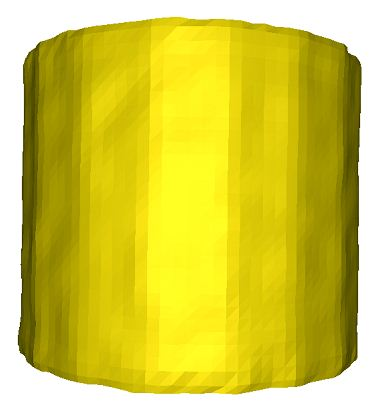
\includegraphics[width = 1.8cm]{results/Prism0.1/snapshot03.jpg}}
%\subfigure
%{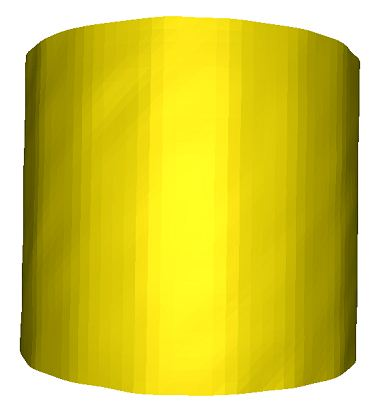
\includegraphics[width = 1.8cm]{results/Prism0.1/snapshot04.jpg}}
%\subfigure
%{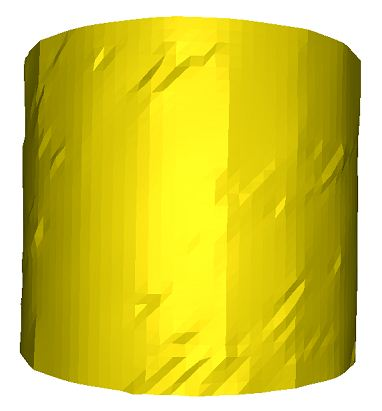
\includegraphics[width = 1.8cm]{results/Prism0.1/snapshot05.jpg}}
%\subfigure
%{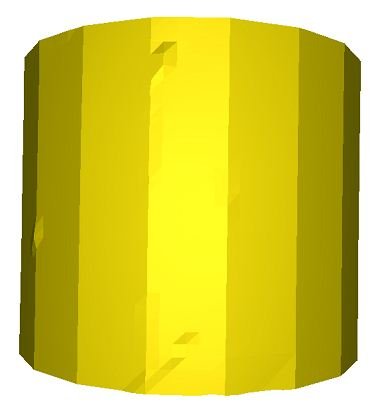
\includegraphics[width = 1.8cm]{results/Prism0.1/snapshot06.jpg}}
%\subfigure
%{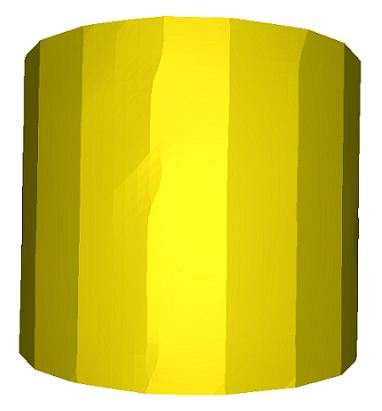
\includegraphics[width = 1.8cm]{results/Prism0.1/snapshot07.jpg}}
%\subfigure
%{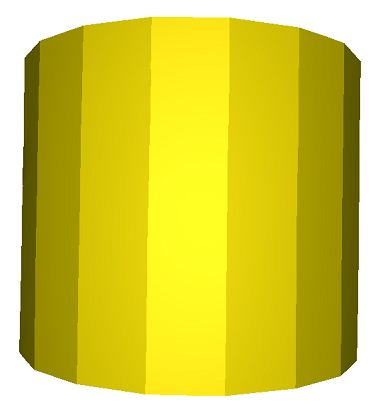
\includegraphics[width = 1.8cm]{results/Prism0.1/snapshot08.jpg}}
%\\
%\vspace{-1.2mm}
%
%\subfigure
%{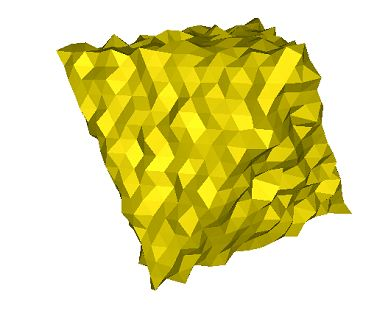
\includegraphics[width = 1.8cm]{results/Octahedron0.3/snapshot00.jpg}}
%\subfigure
%{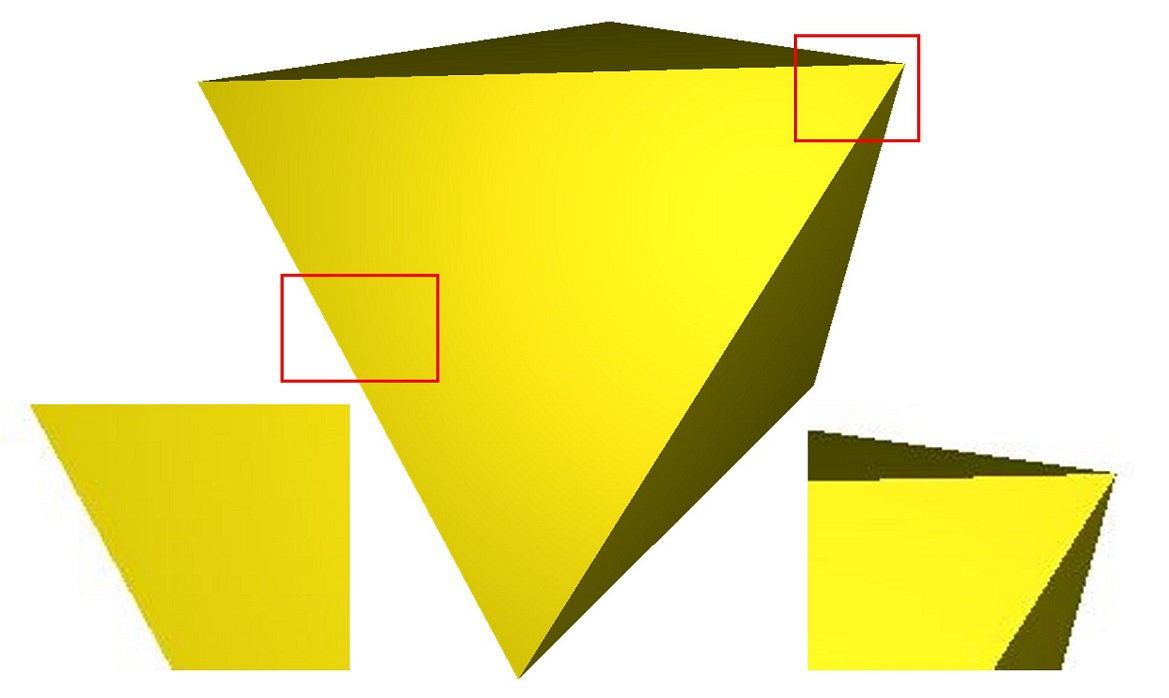
\includegraphics[width = 1.8cm]{results/Octahedron0.3/snapshot01.jpg}}
%\subfigure
%{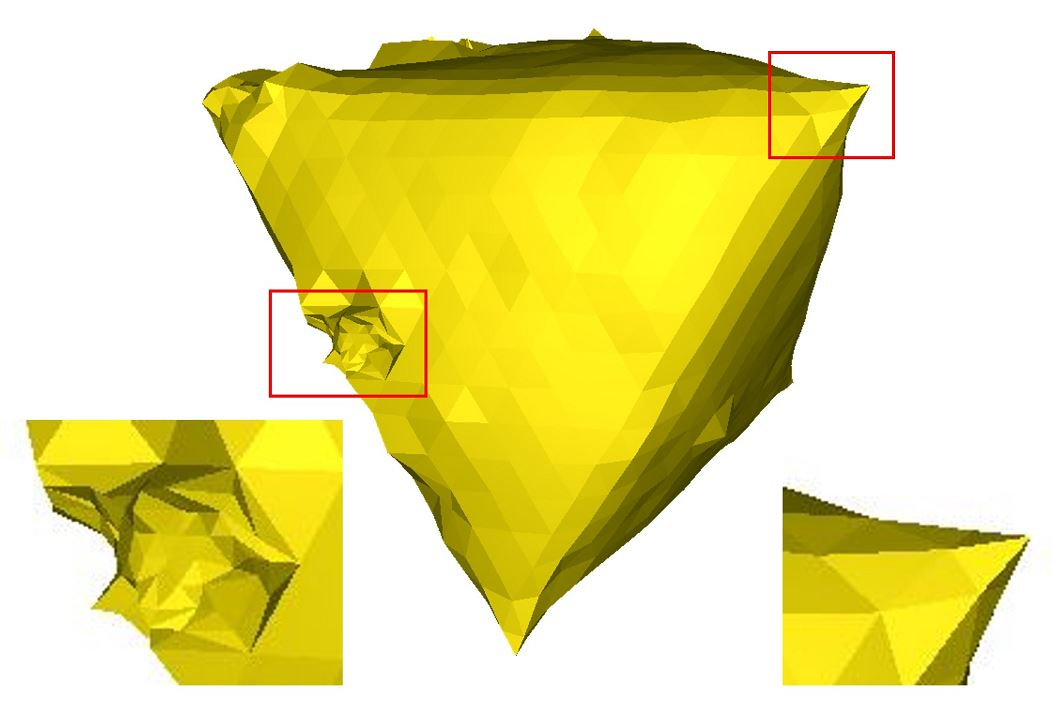
\includegraphics[width = 1.8cm]{results/Octahedron0.3/snapshot02.jpg}}
%\subfigure
%{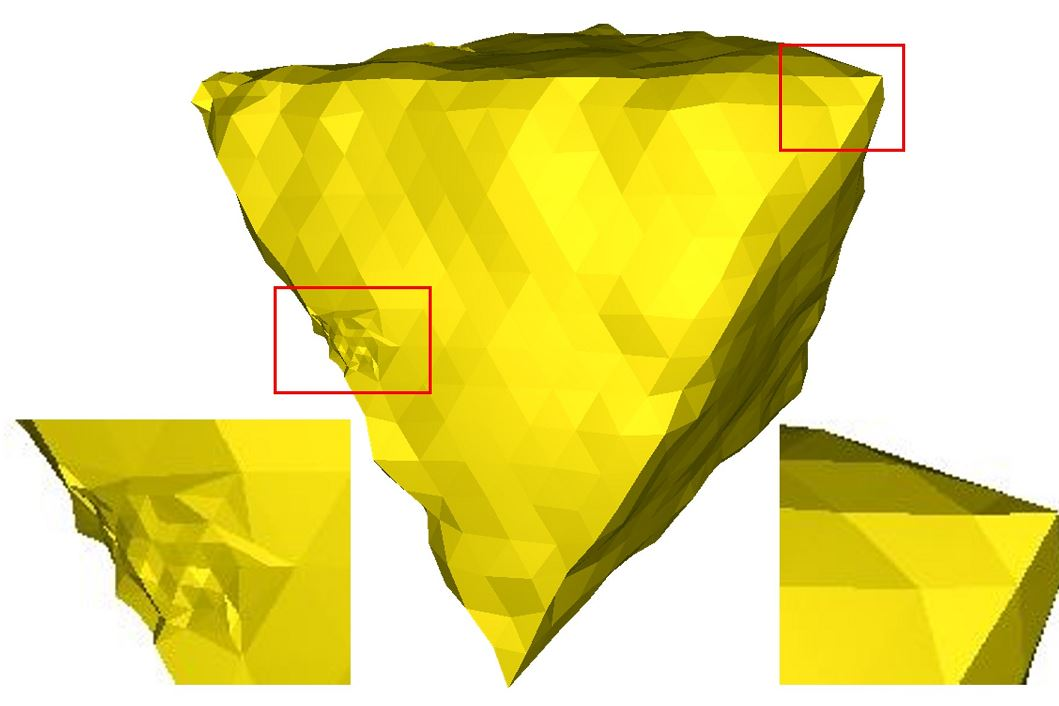
\includegraphics[width = 1.8cm]{results/Octahedron0.3/snapshot03.jpg}}
%\subfigure
%{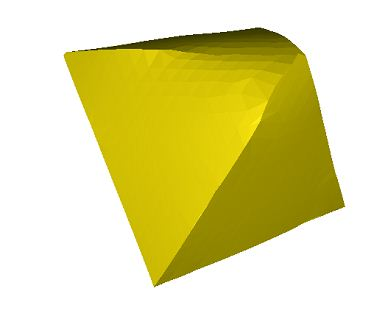
\includegraphics[width = 1.8cm]{results/Octahedron0.3/snapshot04.jpg}}
%\subfigure
%{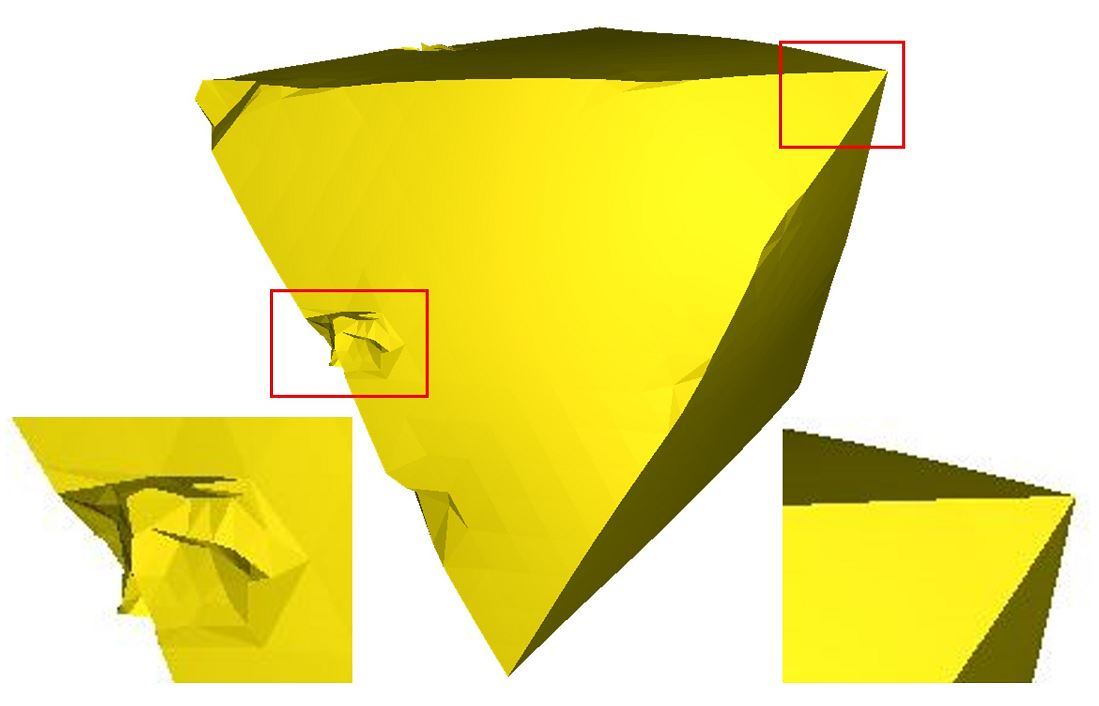
\includegraphics[width = 1.8cm]{results/Octahedron0.3/snapshot05.jpg}}
%\subfigure
%{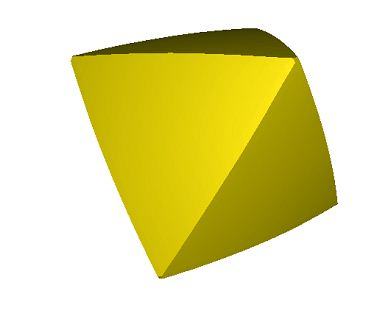
\includegraphics[width = 1.8cm]{results/Octahedron0.3/snapshot06.jpg}}
%\subfigure
%{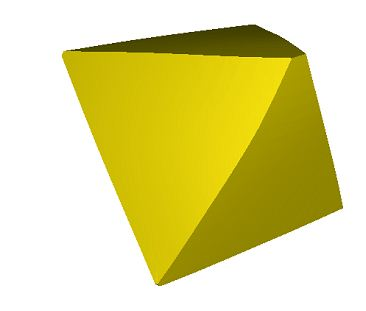
\includegraphics[width = 1.8cm]{results/Octahedron0.3/snapshot07.jpg}}
%\subfigure
%{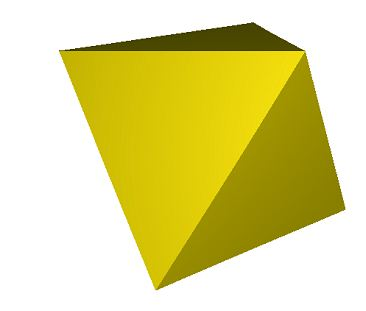
\includegraphics[width = 1.8cm]{results/Octahedron0.3/snapshot08.jpg}}
%\caption{ Comparisons with other methods on synthetic meshes. One with weak edges and the other with sharp corners.
%(a) The noisy mesh( Gaussian noise, $\sigma_E = 0.1$ and 0.3 respectively ). (b) The original mesh.
%(c-i) The results of Fleishman et al~\cite{fleishman2003bilateral},
%Jones et al~\cite{jones2003non}, Sun et al~\cite{sun2007fast}, Zheng et al~\cite{zheng2011bilateral}(l), He et al~\cite{he2013mesh}, Zhang et al~\cite{Zhang2015Filter} and our result separately.}
%\label{Fig:oct_prism}
%\end{figure*}

\begin{figure*}
\centering

\subfigure
{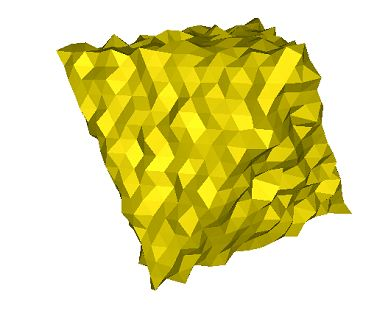
\includegraphics[width = 1.8cm]{results/Octahedron0.3/snapshot00.jpg}}
\subfigure
{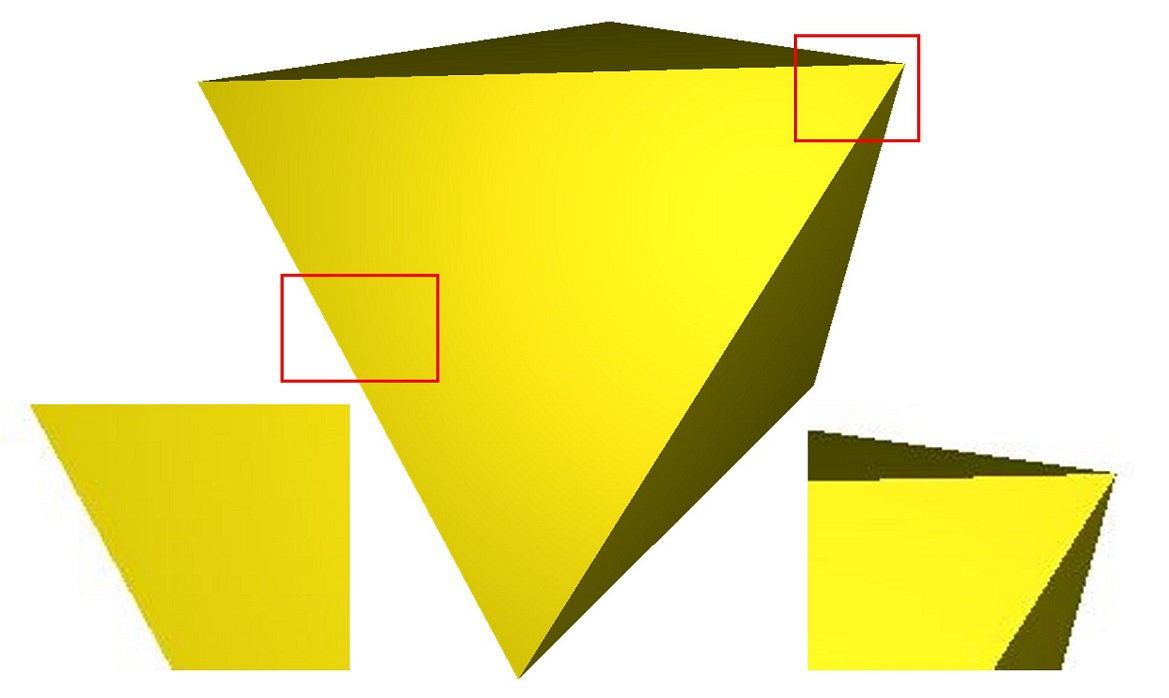
\includegraphics[width = 1.8cm]{results/Octahedron0.3/snapshot01.jpg}}
\subfigure
{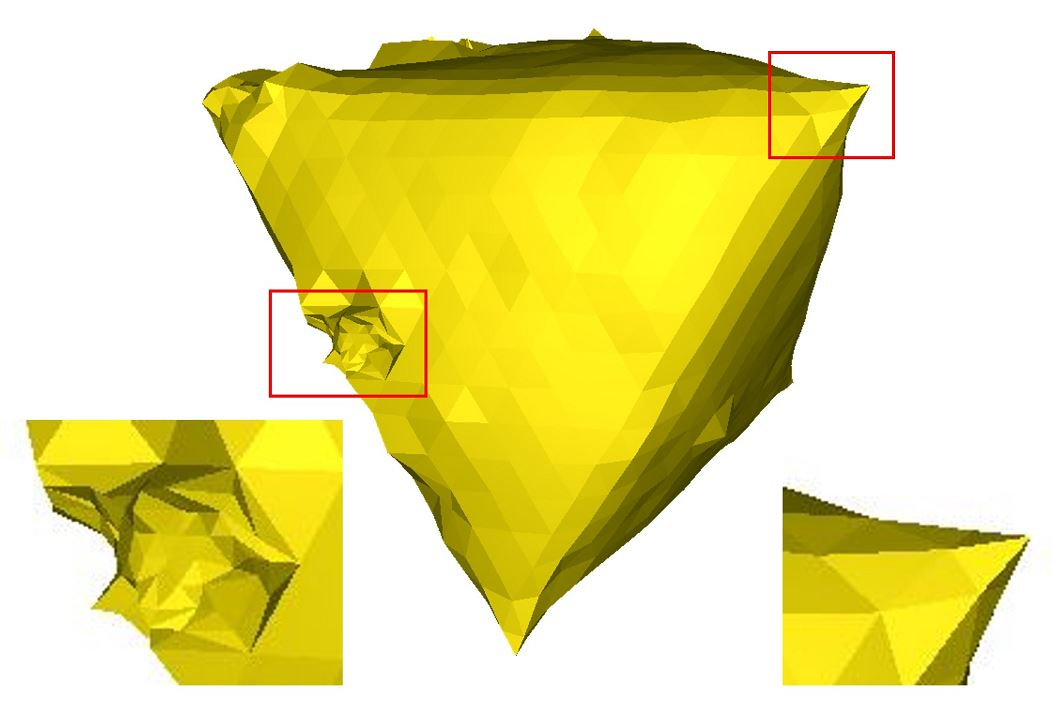
\includegraphics[width = 1.8cm]{results/Octahedron0.3/snapshot02.jpg}}
\subfigure
{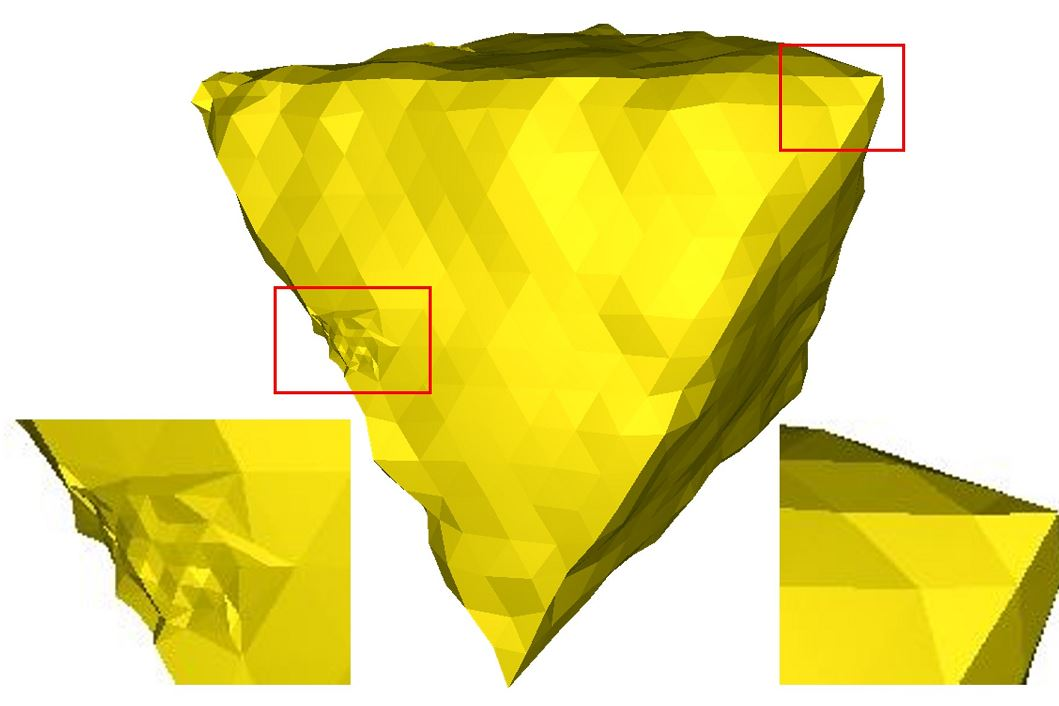
\includegraphics[width = 1.8cm]{results/Octahedron0.3/snapshot03.jpg}}
\subfigure
{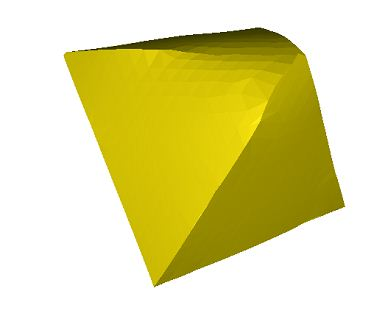
\includegraphics[width = 1.8cm]{results/Octahedron0.3/snapshot04.jpg}}
\subfigure
{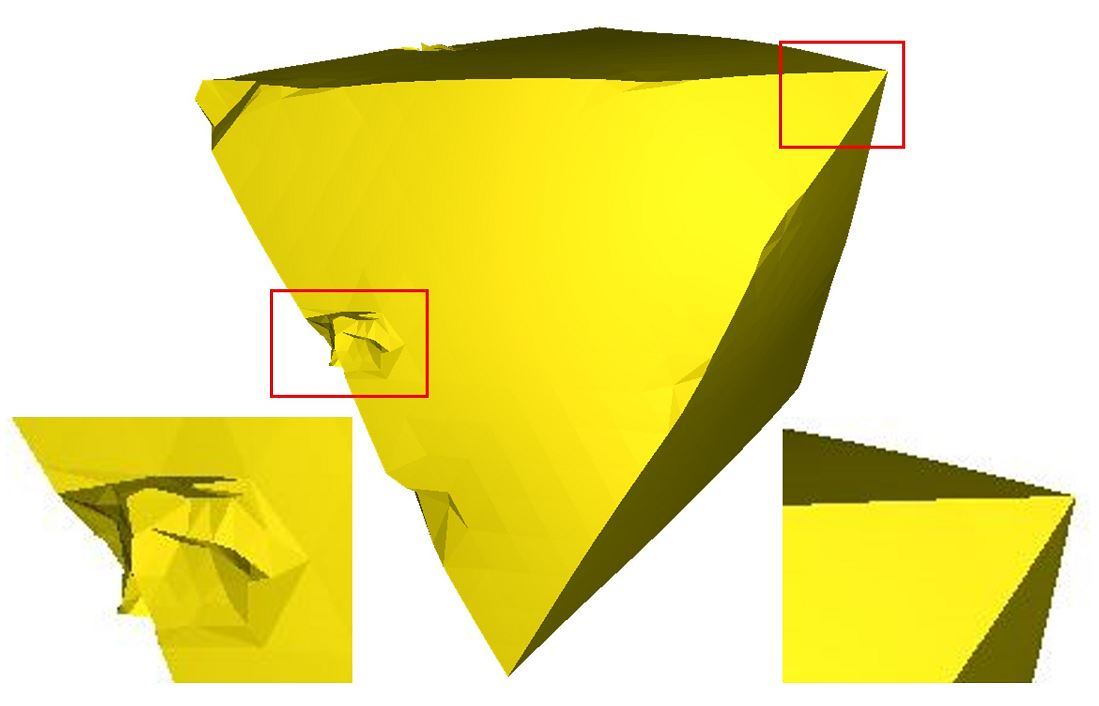
\includegraphics[width = 1.8cm]{results/Octahedron0.3/snapshot05.jpg}}
\subfigure
{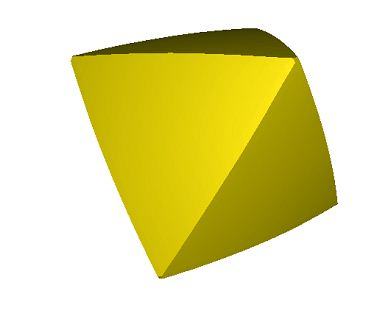
\includegraphics[width = 1.8cm]{results/Octahedron0.3/snapshot06.jpg}}
\subfigure
{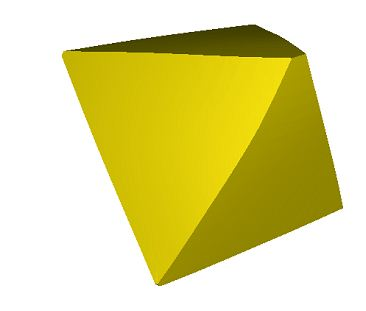
\includegraphics[width = 1.8cm]{results/Octahedron0.3/snapshot07.jpg}}
\subfigure
{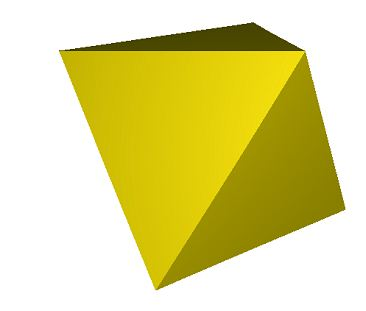
\includegraphics[width = 1.8cm]{results/Octahedron0.3/snapshot08.jpg}}
\\
\vspace{-1.2mm}

\subfigure
{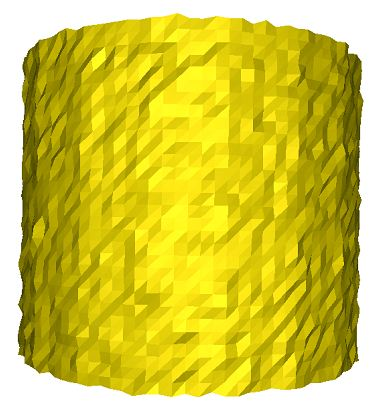
\includegraphics[width = 1.8cm]{results/Prism0.1/snapshot00.jpg}}
\subfigure
{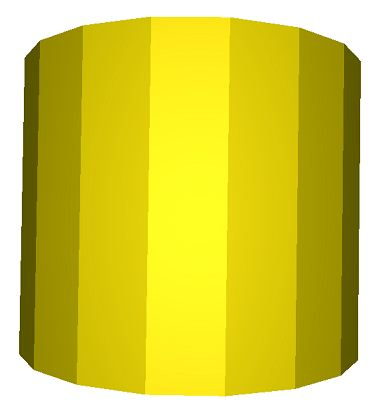
\includegraphics[width = 1.8cm]{results/Prism0.1/snapshot01.jpg}}
\subfigure
{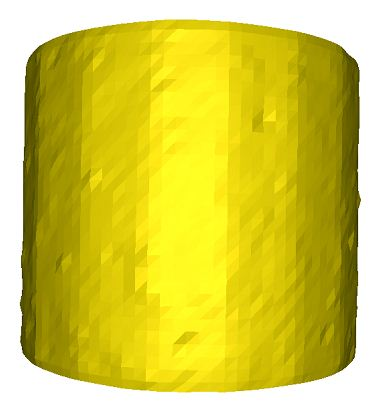
\includegraphics[width = 1.8cm]{results/Prism0.1/snapshot02.jpg}}
\subfigure
{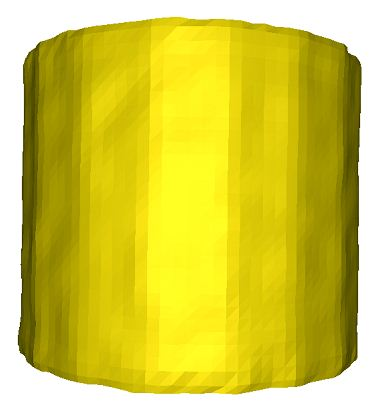
\includegraphics[width = 1.8cm]{results/Prism0.1/snapshot03.jpg}}
\subfigure
{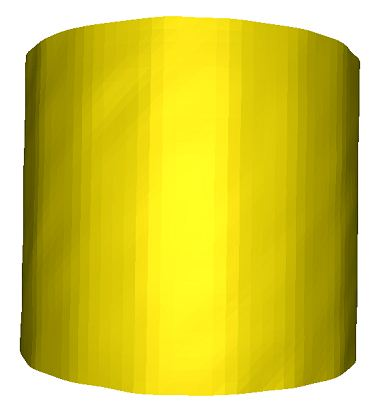
\includegraphics[width = 1.8cm]{results/Prism0.1/snapshot04.jpg}}
\subfigure
{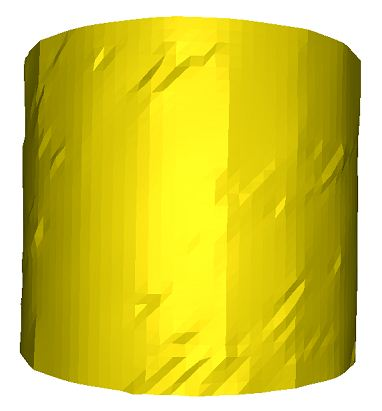
\includegraphics[width = 1.8cm]{results/Prism0.1/snapshot05.jpg}}
\subfigure
{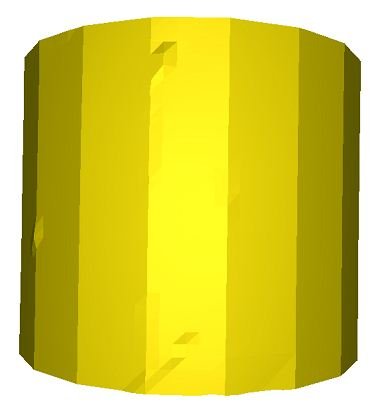
\includegraphics[width = 1.8cm]{results/Prism0.1/snapshot06.jpg}}
\subfigure
{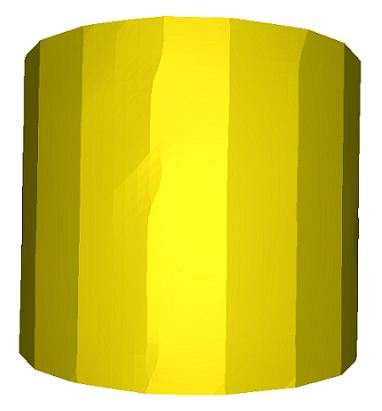
\includegraphics[width = 1.8cm]{results/Prism0.1/snapshot07.jpg}}
\subfigure
{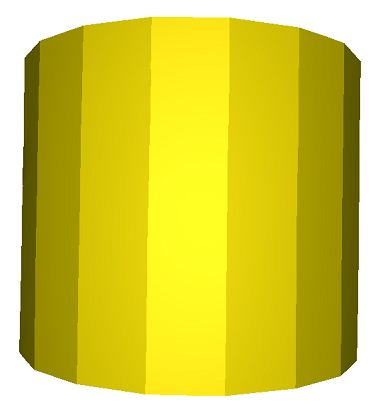
\includegraphics[width = 1.8cm]{results/Prism0.1/snapshot08.jpg}}
\\
\vspace{-1.2mm}

\subfigure
{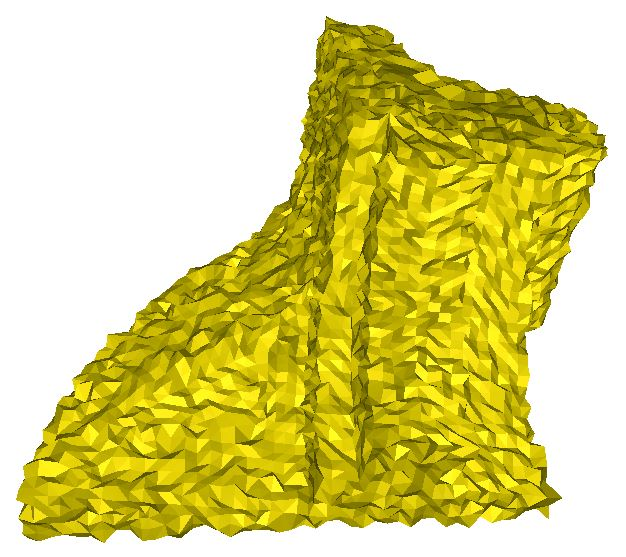
\includegraphics[width = 1.8cm]{results/Fandisk0.3/snapshot00.jpg}}
\subfigure
{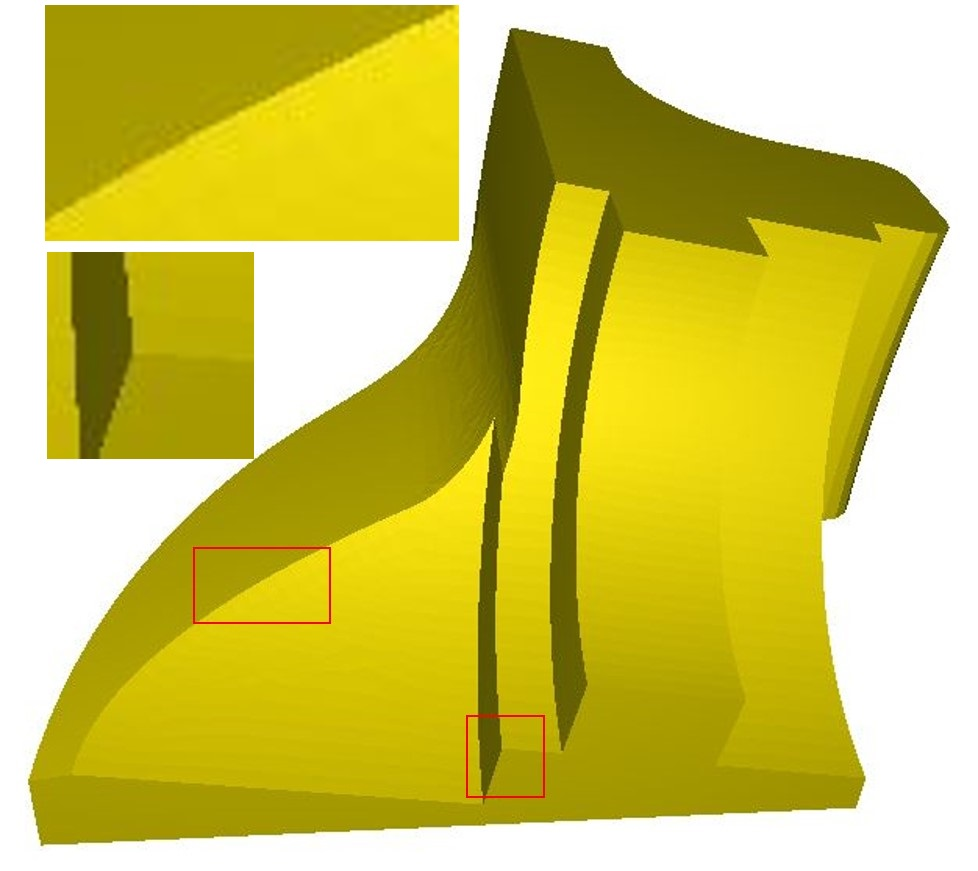
\includegraphics[width = 1.8cm]{results/Fandisk0.3/snapshot01.jpg}}
\subfigure
{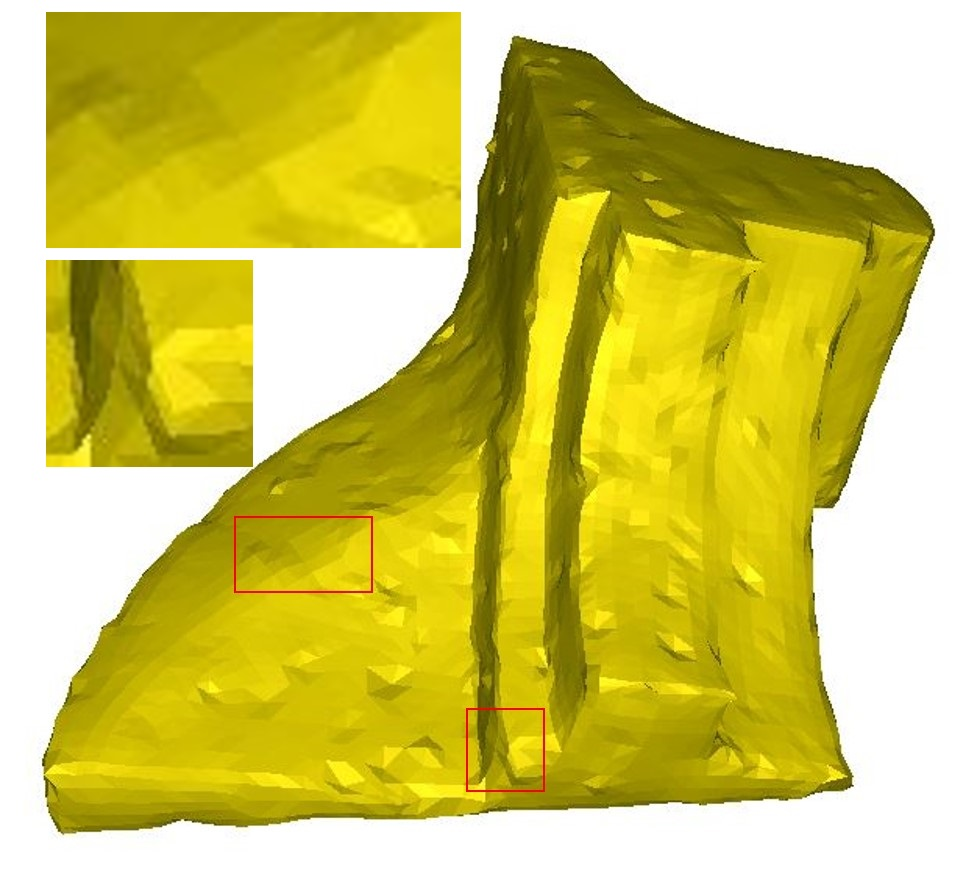
\includegraphics[width = 1.8cm]{results/Fandisk0.3/snapshot02.jpg}}
\subfigure
{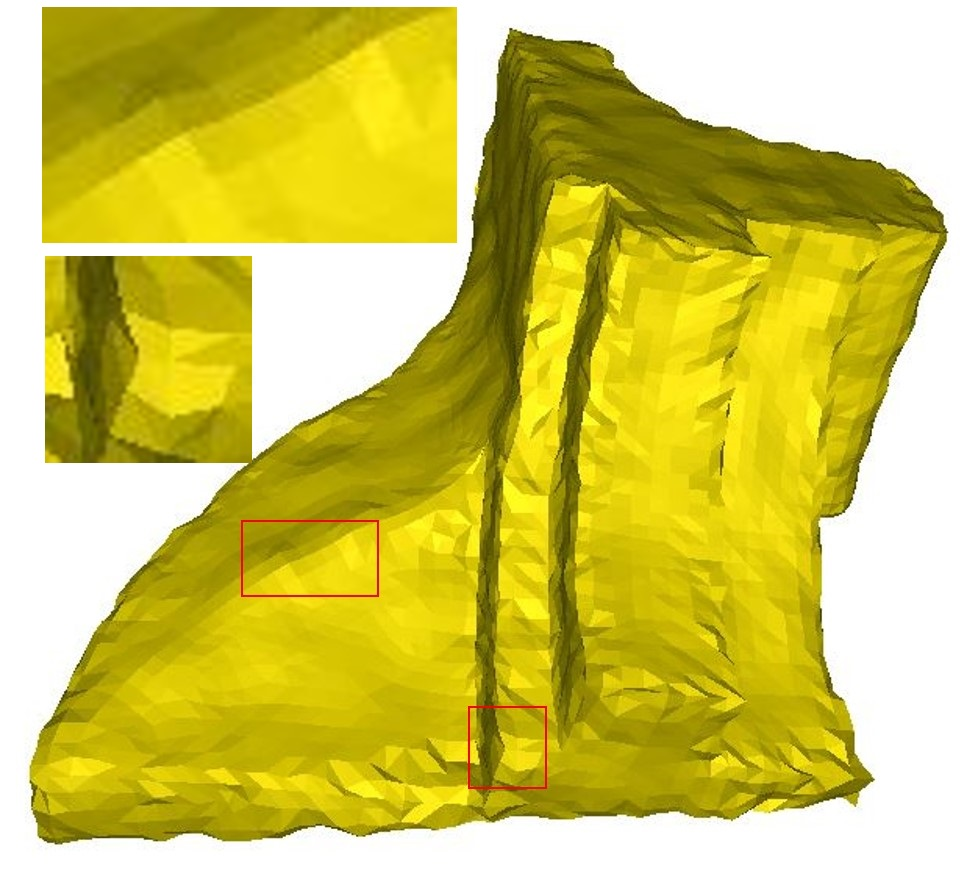
\includegraphics[width = 1.8cm]{results/Fandisk0.3/snapshot03.jpg}}
\subfigure
{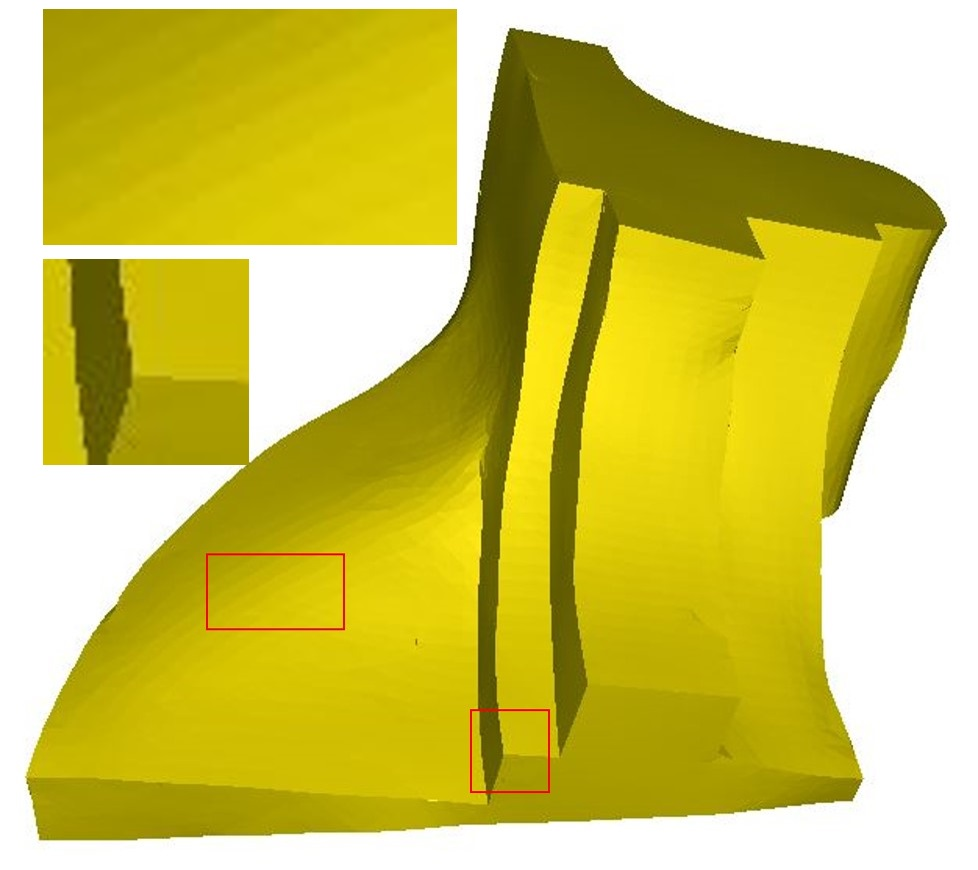
\includegraphics[width = 1.8cm]{results/Fandisk0.3/snapshot04.jpg}}
\subfigure
{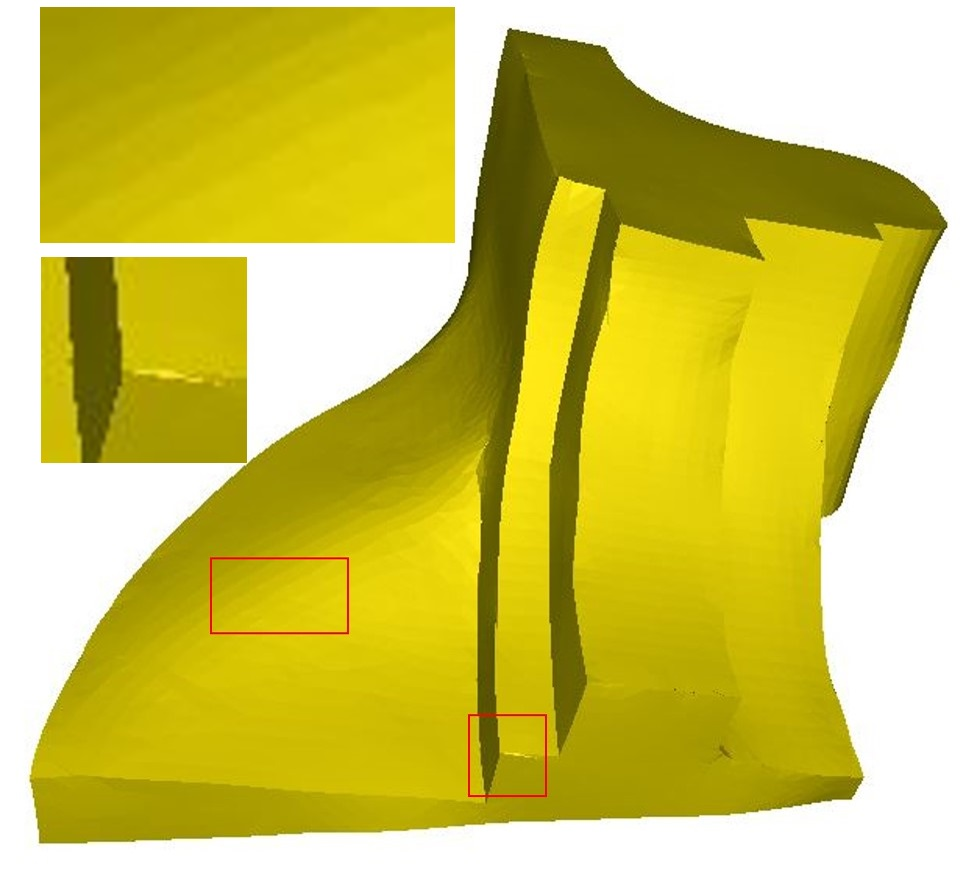
\includegraphics[width = 1.8cm]{results/Fandisk0.3/snapshot05.jpg}}
\subfigure
{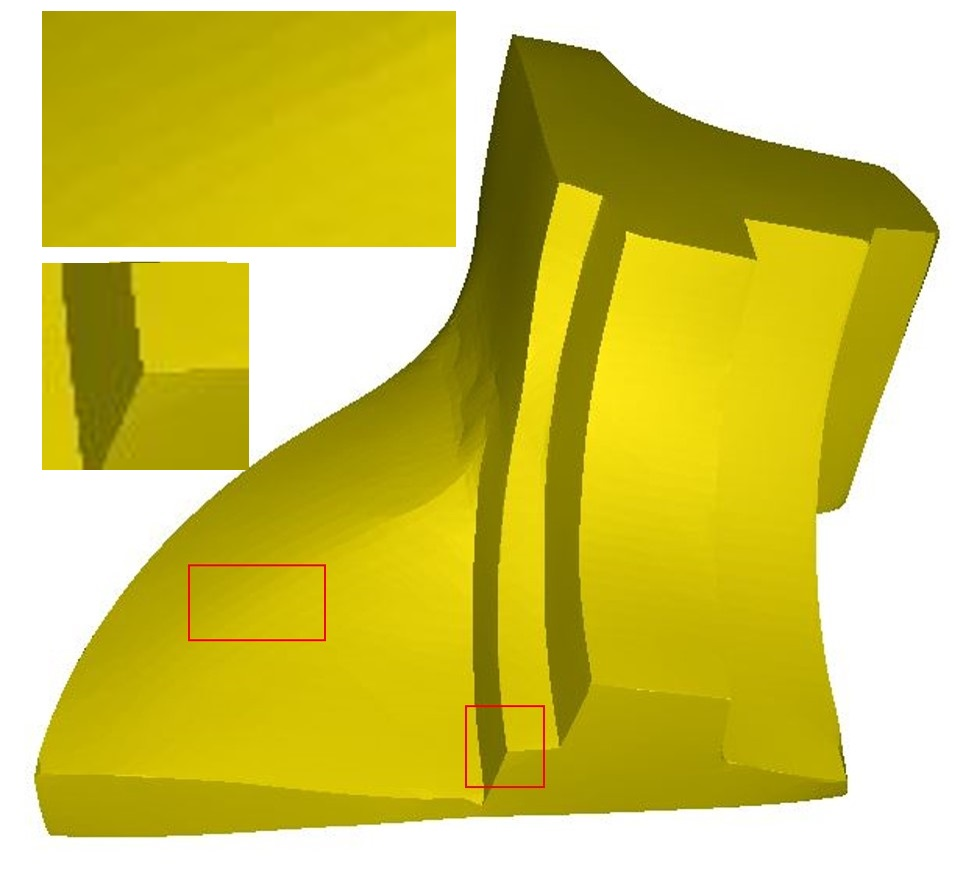
\includegraphics[width = 1.8cm]{results/Fandisk0.3/snapshot06.jpg}}
\subfigure
{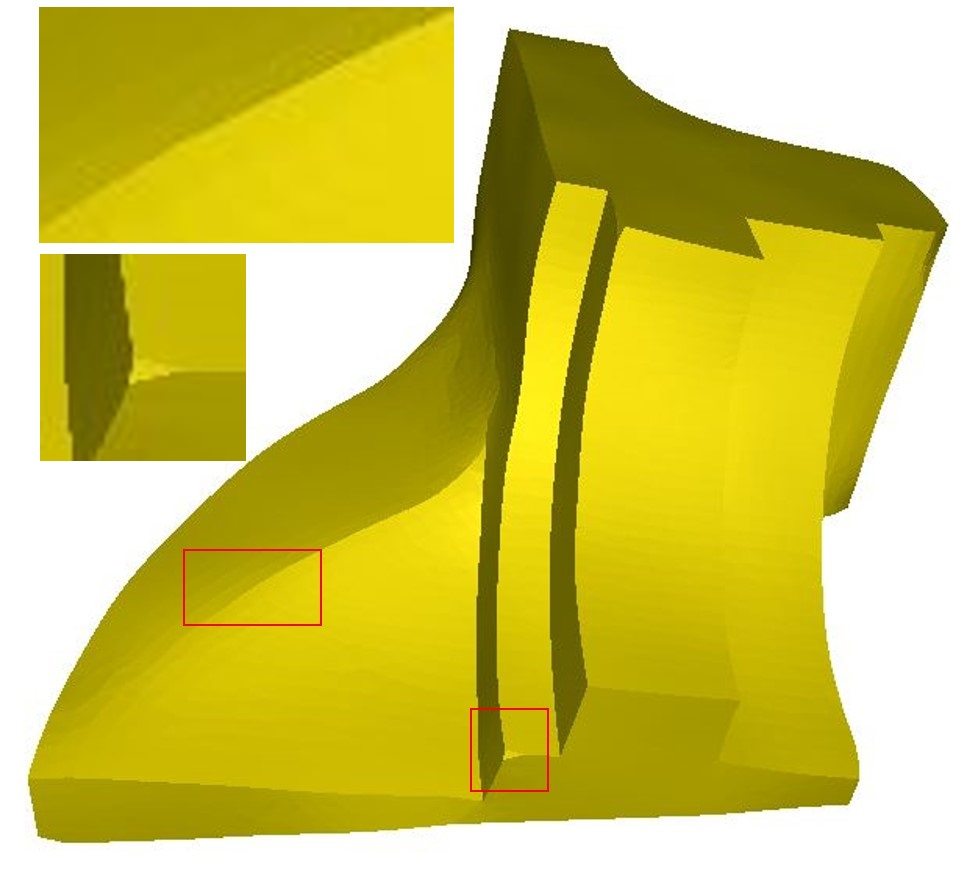
\includegraphics[width = 1.8cm]{results/Fandisk0.3/snapshot07.jpg}}
\subfigure
{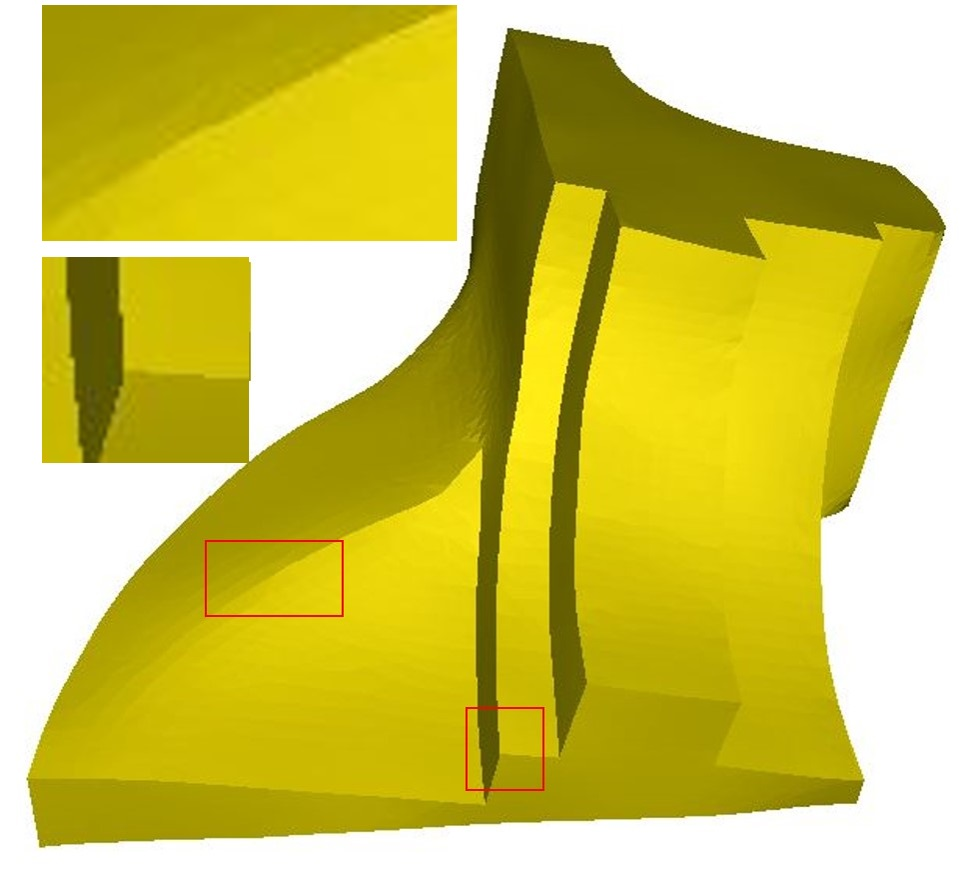
\includegraphics[width = 1.8cm]{results/Fandisk0.3/snapshot08.jpg}}
\\
\vspace{-1.2mm}

\subfigure
{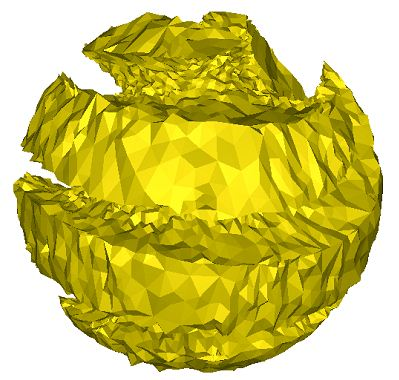
\includegraphics[width = 1.8cm]{results/Sphere0.3/snapshot00.jpg}}
\subfigure
{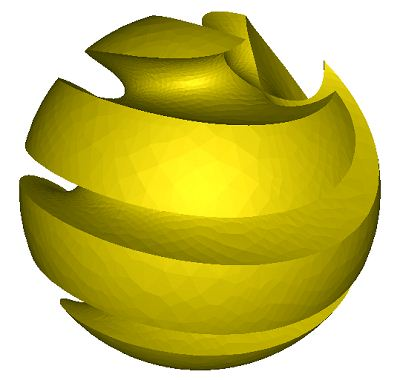
\includegraphics[width = 1.8cm]{results/Sphere0.3/snapshot01.jpg}}
\subfigure
{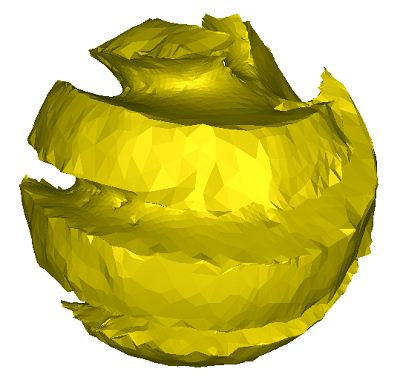
\includegraphics[width = 1.8cm]{results/Sphere0.3/snapshot02.jpg}}
\subfigure
{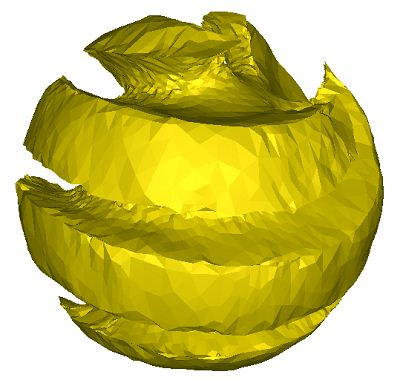
\includegraphics[width = 1.8cm]{results/Sphere0.3/snapshot03.jpg}}
\subfigure
{\includegraphics[width = 1.8cm]{results/Sphere0.3/snapshot04.jpg}}
\subfigure
{\includegraphics[width = 1.8cm]{results/Sphere0.3/snapshot05.jpg}}
\subfigure
{\includegraphics[width = 1.8cm]{results/Sphere0.3/snapshot06.jpg}}
\subfigure
{\includegraphics[width = 1.8cm]{results/Sphere0.3/snapshot07.jpg}}
\subfigure
{\includegraphics[width = 1.8cm]{results/Sphere0.3/snapshot08.jpg}}
\\
\vspace{-1.2mm}

\subfigure
{\includegraphics[width = 1.8cm]{results/Bunny0.2/snapshot00.jpg}}
\subfigure
{\includegraphics[width = 1.8cm]{results/Bunny0.2/snapshot01.jpg}}
\subfigure
{\includegraphics[width = 1.8cm]{results/Bunny0.2/snapshot02.jpg}}
\subfigure
{\includegraphics[width = 1.8cm]{results/Bunny0.2/snapshot03.jpg}}
\subfigure
{\includegraphics[width = 1.8cm]{results/Bunny0.2/snapshot04.jpg}}
\subfigure
{\includegraphics[width = 1.8cm]{results/Bunny0.2/snapshot05.jpg}}
\subfigure
{\includegraphics[width = 1.8cm]{results/Bunny0.2/snapshot06.jpg}}
\subfigure
{\includegraphics[width = 1.8cm]{results/Bunny0.2/snapshot07.jpg}}
\subfigure
{\includegraphics[width = 1.8cm]{results/Bunny0.2/snapshot08.jpg}}
\\
\vspace{-1.2mm}

\subfigure
{\includegraphics[width = 1.8cm]{results/Julius0.2/snapshot00.jpg}}
\subfigure
{\includegraphics[width = 1.8cm]{results/Julius0.2/snapshot01.jpg}}
\subfigure
{\includegraphics[width = 1.8cm]{results/Julius0.2/snapshot02.jpg}}
\subfigure
{\includegraphics[width = 1.8cm]{results/Julius0.2/snapshot03.jpg}}
\subfigure
{\includegraphics[width = 1.8cm]{results/Julius0.2/snapshot04.jpg}}
\subfigure
{\includegraphics[width = 1.8cm]{results/Julius0.2/snapshot05.jpg}}
\subfigure
{\includegraphics[width = 1.8cm]{results/Julius0.2/snapshot06.jpg}}
\subfigure
{\includegraphics[width = 1.8cm]{results/Julius0.2/snapshot07.jpg}}
\subfigure
{\includegraphics[width = 1.8cm]{results/Julius0.2/snapshot08.jpg}}
\caption{ Comparisons with other methods on synthetic meshes with additive Gaussian noise. The results are from left to right noisy mesh, original mesh
, Fleishman et al~\cite{fleishman2003bilateral}, Jones et al~\cite{jones2003non}, Sun et al~\cite{sun2007fast},
Zheng et al~\cite{zheng2011bilateral}(l), He et al~\cite{he2013mesh}, Zhang et al~\cite{Zhang2015Filter} and our result separately.
The intensity $\sigma_E$ of the noise is from the top to bottom 0.3, 0.1, 0.3, 0.3, 0.2 and 0.2.}
\label{Fig:datasets}
\end{figure*}


\begin{figure*}
\centering

\subfigure
{\includegraphics[width = 1.8cm]{results/Block0.4/snapshot00.jpg}}
\subfigure
{\includegraphics[width = 1.8cm]{results/Block0.4/snapshot01.jpg}}
\subfigure
{\includegraphics[width = 1.8cm]{results/Block0.4/snapshot02.jpg}}
\subfigure
{\includegraphics[width = 1.8cm]{results/Block0.4/snapshot03.jpg}}
\subfigure
{\includegraphics[width = 1.8cm]{results/Block0.4/snapshot04.jpg}}
\subfigure
{\includegraphics[width = 1.8cm]{results/Block0.4/snapshot05.jpg}}
\subfigure
{\includegraphics[width = 1.8cm]{results/Block0.4/snapshot06.jpg}}
\subfigure
{\includegraphics[width = 1.8cm]{results/Block0.4/snapshot07.jpg}}
\subfigure
{\includegraphics[width = 1.8cm]{results/Block0.4/snapshot08.jpg}}
\\
\vspace{-1.2mm}

\subfigure
{\includegraphics[width = 1.8cm]{results/TwelveIm0.5/snapshot00.jpg}}
\subfigure
{\includegraphics[width = 1.8cm]{results/TwelveIm0.5/snapshot01.jpg}}
\subfigure
{\includegraphics[width = 1.8cm]{results/TwelveIm0.5/snapshot02.jpg}}
\subfigure
{\includegraphics[width = 1.8cm]{results/TwelveIm0.5/snapshot03.jpg}}
\subfigure
{\includegraphics[width = 1.8cm]{results/TwelveIm0.5/snapshot04.jpg}}
\subfigure
{\includegraphics[width = 1.8cm]{results/TwelveIm0.5/snapshot05.jpg}}
\subfigure
{\includegraphics[width = 1.8cm]{results/TwelveIm0.5/snapshot06.jpg}}
\subfigure
{\includegraphics[width = 1.8cm]{results/TwelveIm0.5/snapshot07.jpg}}
\subfigure
{\includegraphics[width = 1.8cm]{results/TwelveIm0.5/snapshot08.jpg}}
\caption{ Comparisons with other methods on synthetic meshes. One mesh with non-uniform sampling and the Gaussian noise intensity is $\sigma_E = 0.4$, the other mesh with impulsive noise and the intensity is $\sigma_E = 0.5$. The results are from left to right noisy mesh, original mesh
, Fleishman et al~\cite{fleishman2003bilateral}, Jones et al~\cite{jones2003non}, Sun et al~\cite{sun2007fast},
Zheng et al~\cite{zheng2011bilateral}(l), He et al~\cite{he2013mesh}, Zhang et al~\cite{Zhang2015Filter} and our result separately.}
\label{Fig:special}
\end{figure*}

Our method has four parameters: the number of normal filtering iterations $k_{iter}$,
the number of iterations $v_{iter}$ for vertex update,
choosing a radius parameter $r$ determined the geometrical neighborhood,
and the standard variance parameters $\sigma_s$ and $\sigma_r$, for the two difference between normals, respectively.
In our experiments, we find that $k_{iter}\leq80$ and $v_{iter}\leq5$ are enough for achieving satisfactory results.
For all results in this paper, we set the same value to $\sigma_s$ and $\sigma_r$ for employing the filtering unless stated otherwise.
And when their values are between 0.2 and 0.8, a good experimental result can be achieved.
Later, we will introduce the function of the standard variance parameters.
In addition, we choose $r\in[2d, 6d]$ where $d$ is the average distance between neighboring face centroids across the whole mesh.
For CAD model, a bigger $r$ will make a better results.
The reason is that some one of six regions provides more reliable normal estimation.


\subsection{Results and comparisons}

In the following, we compare our denoising results with other methods on synthetic noisy meshes and real meshes.

We generate the synthetic meshes though adding noise to the vertices of a ground truth mesh along the vertex normals.
The intensity of the noise is defined by a relative standard deviation $\sigma_E = \sigma / E_{mean}$,
where $\sigma$ is the standard deviation of the Gaussian function and $E_{mean}$ is the average edge length of the ground truth mesh.
For a fair comparison, for each method we fine tune the parameters to produce the best results in their parameter space.
And furthermore, for synthetic meshes, we also evaluate two quantitative metrics about vertex-based and normal-based mesh-to-mesh error metric
separately introduced in papers~\cite{belyaev2003comparison} and~\cite{nehorai2000performance} to analyze the difference between our results and others.
These two metrics measure mean deviations about vertex and face between denoised mesh and true mesh.

The vertex-based error metric is
\begin{equation}
\label{Eq:vertexerror}
E_v = \sqrt{\frac{1}{3 A(M^{'})}\sum_{P^{'} \in M^{'}} A(P^{'}) dist(P^{'}, M)^2}\, ,
\end{equation}
where $M$ and $M^{'}$ reference original noiseless mesh and denoised mesh respectively, $P^{'}$ is a vertex of $M^{'}$
and $dist(P^{'}, M)$ defines the distance between $P^{'}$ and a triangle of $M$ which is closest to $P^{'}$.

The normal-based error metric is used to reveal the average angle offset which is defined as follows
\begin{equation}
\label{Eq:vertexerror}
E_n = \sum_{f^{'} \in M^{'}, f \in M} angle(\mathbf{n^{'}}, \mathbf{n}) / N\, ,
\end{equation}
where $f^{'}$ and $f$ are triangle faces of $M^{'}$ and $M$ respectively,
$\mathbf{n^{'}}$ and $\mathbf{n}$ reference the normal of $f^{'}$ and $f$,
$angle(\mathbf{n^{'}}, \mathbf{n})$ defines the angle between $\mathbf{n^{'}}$ and $\mathbf{n}$
and the last $N$ is the number of triangle faces of a mesh.

{\bfseries Comparison with other methods on the synthetic meshes.}
Figure~\ref{Fig:oct_prism} shows the effectiveness of our method on preserving weak edges and sharp corners.
From the results of first line on a noisy octahedron, the approaches of Fleishman et al~\cite{fleishman2003bilateral} and Jones et al~\cite{jones2003non}
can not well preserve the strong edges, because the spatial weight weaken the strength of filtering.
While the rest of methods have the ability to maintain the mesh edge structure, they can not well deal with the sharp corner.
The main reason is that the methods of Sun et al~\cite{sun2007fast} and Zheng et al~\cite{zheng2011bilateral}(l) easily smooth the sharp corner,
The approaches of He et al~\cite{he2013mesh} and Zhang et al~\cite{Zhang2015Filter} are prone to ambiguity.
Because our method divide the neighbor sets, it can well preserve the sharp corner and edge.
The second line is the denoised results on a prism with 18 edges with the Gaussian noise intensity $\sigma_E = 0.1$.
Other methods can not well restore these weak edges and easily smooth them.
We do well in the two models not only because our denoised method but also the function of six regions which give a better estimation in the structure of local mesh.

The models in figures~\ref{Fig:datasets} and ~\ref{Fig:special} all selected from~\cite{Zhang2015Filter}.
For most of models, our method achieves better results than others according to the table~\ref{Tab:1}.
The detail of parameters can be found in the supplementary material.

In the figure~\ref{Fig:special}, we show our method also can deal with different kinds of noise.
From the vision, our method almost obtains the similar results comparing with Zhang et al~\cite{Zhang2015Filter}.
However, according to the table~\ref{Tab:1}, our method works well.

{\bfseries Comparison with other methods on the real noisy meshes.}
Figure~\ref{Fig:TrueMesh} witnesses the denoised effectiveness on real world 3D objects.

Table~\ref{Tab:Time} provides the timing of our approach for the shown examples, on a PC with an Intel Core $i7-4790K$.


\begin{table}
\caption{Time consumption for different results. }
\vspace{2mm}
\label{Tab:Time}
\begin{center}
\begin{tabular}{|c|c|c|c|c|}
\hline
\rule[-1ex]{0pt}{3.5ex} Model & Vertics & Faces & Time(s) & $k_{iter}$ \\
\hline\hline
\rule[-1ex]{0pt}{3.5ex} Fandisk (Fig~\ref{Fig:datasets}) & Vertices & Faces & Time(s) & $k_{iter}$ \\
\hline
\rule[-1ex]{0pt}{3.5ex} Fandisk (Fig~\ref{Fig:datasets}) & Vertices & Faces & Time(s) & $k_{iter}$ \\
\hline
\rule[-1ex]{0pt}{3.5ex} Fandisk (Fig~\ref{Fig:datasets}) & Vertices & Faces & Time(s) & $k_{iter}$ \\
\hline
\rule[-1ex]{0pt}{3.5ex} Fandisk (Fig~\ref{Fig:datasets}) & Vertices & Faces & Time(s) & $k_{iter}$ \\
\hline
\rule[-1ex]{0pt}{3.5ex} Fandisk (Fig~\ref{Fig:datasets}) & Vertices & Faces & Time(s) & $k_{iter}$ \\
\hline
\rule[-1ex]{0pt}{3.5ex} Fandisk (Fig~\ref{Fig:datasets}) & Vertices & Faces & Time(s) & $k_{iter}$ \\
\hline
\rule[-1ex]{0pt}{3.5ex} Fandisk (Fig~\ref{Fig:datasets}) & Vertices & Faces & Time(s) & $k_{iter}$ \\
\hline
\rule[-1ex]{0pt}{3.5ex} Fandisk (Fig~\ref{Fig:datasets}) & Vertices & Faces & Time(s) & $k_{iter}$ \\
\hline
\rule[-1ex]{0pt}{3.5ex} Fandisk (Fig~\ref{Fig:datasets}) & Vertices & Faces & Time(s) & $k_{iter}$ \\
\hline
\rule[-1ex]{0pt}{3.5ex} Fandisk (Fig~\ref{Fig:datasets}) & Vertices & Faces & Time(s) & $k_{iter}$ \\
\hline

\end{tabular}
\end{center}
\end{table}



\begin{table*}[ht]
\caption{Quantitative comparisons using two error metrics.}
\vspace{2mm}
\label{Tab:1}
\begin{center}
\begin{tabular}{|c|c|c|c|c|c|c|c|c|} %% this creates eight columns also can be "c" and "r", "|" representative inserting ����
%% |l|l| to left justify each column entry
%% |c|c| to center each column entry
%% use of \rule[]{}{} below opens up each row
\hline
\rule[-1ex]{0pt}{3.5ex}  Model & Error  &  \cite{fleishman2003bilateral}  & \cite{jones2003non} & \cite{sun2007fast} & \cite{zheng2011bilateral}(l) & \cite{he2013mesh} & \cite{Zhang2015Filter} & ours \\
\hline\hline

\rule[-1ex]{0pt}{3.5ex}  \multirow{2}{*}{Prism (Fig~\ref{Fig:datasets})}
& $E_n$ & 4.98 & 4.48 & 3.29 & 3.87 & 0.71 & 0.87 & \textbf{0.46} \\
\cline{2-9}
& $E_v(\times10^{-2})$ & 11.89 & 10.46 & 7.45 & 7.9  & 3.42 & 4.09 & \textbf{2.77}\\
\hline

\rule[-1ex]{0pt}{3.5ex}  \multirow{2}{*}{octahedron (Fig~\ref{Fig:datasets})}
& $E_n$ & 12.81 & 10.65 & 6.85 & 5.27 & 3.33 & 3.36 & \textbf{1.00} \\
\cline{2-9}
& $E_v(\times10^{-3})$ & 28.02 & 14.70 & 10.71 & 6.28 & 10.81 & 4.90 & \textbf{3.02}\\
\hline

\rule[-1ex]{0pt}{3.5ex}  \multirow{2}{*}{Fandisk (Fig~\ref{Fig:datasets})}
& $E_n$ & 9.73 & 9.82 & 4.04 & 3.35 & 5.53 & 2.62 & \textbf{2.27} \\
\cline{2-9}
& $E_v(\times10^{-3})$ & 18.14 & 15.10 & 11.02 & 8.72 & 18.79 & \textbf{6.29} & 6.35\\
\hline

\rule[-1ex]{0pt}{3.5ex}  \multirow{2}{*}{sphere (Fig~\ref{Fig:datasets})}
& $E_n$ & 12.58 & 17.36 & 11.89 & \textbf{6.70} & 12.96 & 10.17 & 7.39 \\
\cline{2-9}
& $E_v(\times10^{-2})$ & 15.51 & 8.46 & 8.88 & 4.48 & 12.41 & 5.65 & \textbf{4.37}\\
\hline

\rule[-1ex]{0pt}{3.5ex}  \multirow{2}{*}{bunny (Fig~\ref{Fig:datasets})}
& $E_n$ & 6.93 & 5.81 & 5.89 & 5.68 & 7.21 & 5.35 & \textbf{5.11} \\
\cline{2-9}
& $E_v(\times10^{-4})$ & 18.36 & 9.24 & 9.98 & 9.35 & 10.65 & 7.61 & \textbf{7.26}\\
\hline

\rule[-1ex]{0pt}{3.5ex}  \multirow{2}{*}{Julius (Fig~\ref{Fig:datasets})}
& $E_n$ & 7.70 & 7.63 & 7.01 & 6.21 & 7.98 & 6.38 & \textbf{6.11} \\
\cline{2-9}
& $E_v(\times10^{-4})$ & 10.58 & 7.71 & 6.49 & \textbf{5.53} & 8.60 & 6.02 & 5.78\\
\hline

\rule[-1ex]{0pt}{3.5ex}  \multirow{2}{*}{block (Fig~\ref{Fig:special})}
& $E_n$ & 12.72 & 13.85 & 5.80 & 5.31 & 4.97 & 3.57 & \textbf{3.02} \\
\cline{2-9}
& $E_v(\times10^{-2})$ & 17.98 & 13.35 & 8.21 & 6.80 & 11.60 & 5.41 & \textbf{4.99}\\
\hline

\rule[-1ex]{0pt}{3.5ex}  \multirow{2}{*}{twelve (Fig~\ref{Fig:special})}
& $E_n$ & 11.72 & 11.09 & 7.45 & 7.37 & 8.46 & 2.75 & \textbf{1.78} \\
\cline{2-9}
& $E_v(\times10^{-3})$ & 20.85 & 17.28 & 12.06 & 12.54  & 20.13 & 6.16 & \textbf{5.23}\\
\hline

%\rule[-1ex]{0pt}{3.5ex}  \multirow{2}{*}{Nicolo}
%& $E_n$ & 8.88 & 7.13 & 6.38 & \textbf{5.80} & 7.58 & 6.50 & 5.93 \\
%\cline{2-9}
%& $E_v(\times10^{-1})$ & 4.60 & 3.33 & 3.18 & 2.59  & 3.48 & 2.61 & \textbf{2.50}\\
%\hline

\end{tabular}
\end{center}
\end{table*}


\begin{figure*}[tb]
\centering
\includegraphics[width = 15.0cm]{results/truemesh.jpg}
\vspace{0.5mm}
\caption{ true mesh.}
\label{Fig:TrueMesh}
\end{figure*}

\subsection{Limitation and discussion}

Figure~\ref{Fig:Convergence} shows the convergence of our method.

\begin{figure}
\centering
\includegraphics[width = 8cm]{results/convergence.jpg}
\vspace{0.5mm}
\caption{ the convergence.}
\label{Fig:Convergence}
\end{figure}

\section{Conclusion}

In this paper, we introduce a intrinsic signal filtering framework for denoising 2D manifold surface.
Intrinsically, our method builds the relation between desired filtering signals and its neighbors, making calculate weights more reasonably.
Other famous filtering algorithm, such as bilateral, geodesic and propagation filters, can be simplified by our algorithm.
Furthermore, we apply our filtering framework to triangular meshes and obtain state-of-the-art performance.
We also propose a simple, fast and effective method for choosing path in the process of intrinsic filtering algorithm instead of geodesic path.
And, the approach for dividing region protects the local mesh structure in a certain extent, further increasing the effectiveness of mesh filter.
Finally, a large number of experiments prove the effectiveness of our method.




{\bfseries Acknowledgements}
